\section{Auswertung}
\label{sec:Auswertung}

\subsection{Beugung am Parallelspalt}
  Für einen 0,15 mm breiten Einfachspalt, der in 1,047 m Entfernung vom Schirm aufgestellt
  wird, wurden die folgenden Messdaten aufgenommen:
  \begin{table}[H]
  \centering
  \caption{Messwerte des Selektivverstärkers}
  \label{tab:mag}
  \begin{tabular}{c c}
   \toprule
    Winkel $\phi$ & Intensität [A]\\
   \midrule
   -0.026     & -2.27e-09    \\
 -0.025       & -2.27e-09    \\
 -0.024       &  7.73e-09    \\
 -0.023       & -2.27e-09    \\
 -0.022       & -2.27e-09    \\
 -0.021       &  7.73e-09    \\
 -0.02        &  1.9773e-07  \\
 -0.019       &  7.73e-09    \\
 -0.018       & -2.27e-09    \\
 -0.017       &  7.73e-09    \\
 -0.016       &  4.9773e-07  \\
 -0.015       &  4.9773e-07  \\
 -0.014       & -2.27e-09    \\
 -0.013       &  7.73e-09    \\
 -0.012       &  9.9773e-07  \\
 -0.011       &  1.49773e-06 \\
 -0.01        &  9.9773e-07  \\
 -0.009       &  4.9773e-07  \\
 -0.008       &  2.49773e-06 \\
 -0.007       &  5.49773e-06 \\
 -0.006       &  4.49773e-06 \\
 -0.005       &  9.9773e-07  \\
 -0.004       &  3.99773e-06 \\
 -0.003       &  2.19977e-05 \\
 -0.002       &  6.09977e-05 \\
 -0.001       &  9.49977e-05 \\
  0           &  0.000129998 \\
  0.001       &  9.49977e-05 \\
  0.002       &  4.39977e-05 \\
  0.003       &  1.29977e-05 \\
  0.004       &  4.99773e-06 \\
  0.005       &  2.99773e-06 \\
  0.006       &  4.99773e-06 \\
  0.007       &  2.49773e-06 \\
  0.008       &  9.9773e-07  \\
  0.009       &  6.9773e-07  \\
  0.01        &  1.49773e-06 \\
  0.011       &  1.49773e-06 \\
  0.012       &  4.9773e-07  \\
  0.013       &  2.4773e-07  \\
  0.014       &  4.9773e-07  \\
  0.015       &  4.9773e-07  \\
  0.016       & -2.27e-09    \\
  0.017       & -2.27e-09    \\
  0.018       &  9.773e-08   \\
  0.019       &  4.4773e-07  \\
  0.02        &  9.773e-08   \\
  0.021       & -2.27e-09    \\
  0.022       & -2.27e-09    \\
  0.023       & -2.27e-09    \\
  0.024       & -2.27e-09    \\
   \bottomrule
  \end{tabular}
 \end{table} 
  Bei diesen wird der Dunkelstrom abgezogen, weshalb manche Werte ins Negative geraten.
  Die Daten werden durch die Funktion \ref{eq:6}
  \begin{equation*}
    I=A_0^2\cdot b^2\cdot (\dfrac{\lambda}{\pi \ b \ \sin{\psi}})^2 \cdot \sin{\pi \ b \ (\sin{\dfrac{\phi}{\lambda}}})^2
  \end{equation*}
  angenähert. Diese ist in Abbildung \ref{fig:plot} dargestellt.
  \begin{figure}
    \centering
    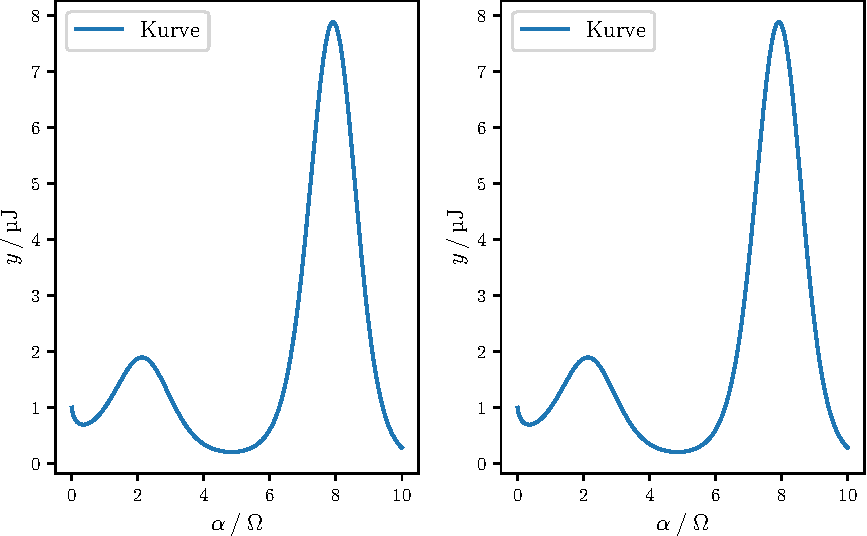
\includegraphics{plot.pdf}
    \caption{Messwerte des Einfachspaltes}
    \label{fig:doppel}
  \end{figure}
  Die für die Koeffizienten ermittelten Werte lauten:
  \begin{align*}
    A_0 = 69.8477 \pm 1.009 \si{\ampere}\\
    b = (157.4 \pm 2.63) \cdot 10^{-6} \si{\metre}
  \end{align*}
  

\subsection{Beugung am Doppelspalt}
  Die gemessenen Werte für den Doppelspalt lauten:
  \begin{table}[H]
    \centering
    \caption{Messwerte des Selektivverstärkers}
    \label{tab:mag}
    \begin{tabular}{c c}
     \toprule
      Winkel $\phi$ & Intensität\\
     \midrule
  -0.026       & 8.99773e-06 \\
 -0.025       & 5.99773e-06 \\
 -0.024       & 4.9773e-07  \\
 -0.023       & 1.49773e-06 \\
 -0.022       & 1.09977e-05 \\
 -0.021       & 1.04977e-05 \\
 -0.02        & 1.49773e-06 \\
 -0.019       & 2.49773e-06 \\
 -0.018       & 1.39977e-05 \\
 -0.017       & 1.69977e-05 \\
 -0.016       & 1.99773e-06 \\
 -0.015       & 2.99773e-06 \\
 -0.014       & 2.04977e-05 \\
 -0.013       & 2.39977e-05 \\
 -0.012       & 4.49773e-06 \\
 -0.011       & 6.49773e-06 \\
 -0.01        & 3.39977e-05 \\
 -0.009       & 5.99977e-05 \\
 -0.008       & 2.99773e-06 \\
 -0.007       & 9.99773e-06 \\
 -0.006       & 2.49977e-05 \\
 -0.005       & 1.44773e-06 \\
 -0.004       & 1.89977e-05 \\
 -0.003       & 4.79977e-05 \\
 -0.002       & 0.000259998 \\
 -0.001       & 0.0023      \\
  3.46945e-18 & 0.003       \\
  0.001       & 0.000469998 \\
  0.002       & 0.000269998 \\
  0.003       & 0.000799998 \\
  0.004       & 7.99977e-05 \\
  0.005       & 1.89977e-05 \\
  0.006       & 2.19977e-05 \\
  0.007       & 8.79977e-05 \\
  0.008       & 2.19977e-05 \\
  0.009       & 1.29977e-05 \\
  0.01        & 6.99773e-06 \\
  0.011       & 4.79977e-05 \\
  0.012       & 1.39977e-05 \\
  0.013       & 7.49773e-06 \\
  0.014       & 5.99773e-06 \\
  0.015       & 9.99773e-06 \\
  0.016       & 5.99773e-06 \\
  0.017       & 3.74773e-06 \\
  0.018       & 1.99773e-06 \\
  0.019       & 6.99773e-06 \\
  0.02        & 4.99773e-06 \\
  0.021       & 1.99773e-06 \\
  0.022       & 9.9773e-07  \\
  0.023       & 6.99773e-06 \\
  0.024       & 2.99773e-06 \\
  \bottomrule
  \end{tabular}
  \end{table}
  Diese Daten wurden anhand der in der Theorie hergeleiteten Formel 
  \begin{equation*}
    I= A_0^2\cdot \cos{\dfrac{\pi\ s \sin{\phi}}{\lambda}}^2 \cdot
    (\dfrac{\lambda}{\pi \ b \sin{\phi}})^2 \cdot (\sin{\dfrac{\pi\ b \sin{\phi}}{\lambda}})^2
  \end{equation*}
  ausgewertet und werden in der folgenden Abbildung dargestellt
  \begin{figure}
    \centering
    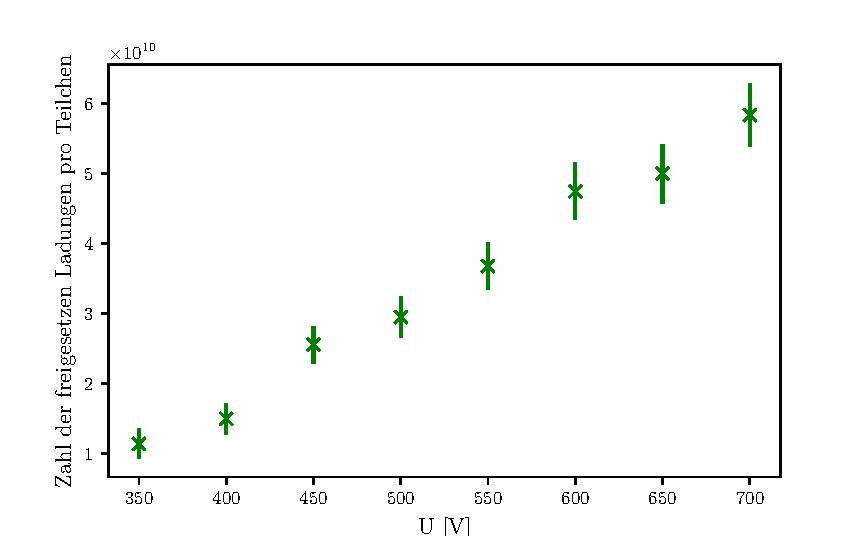
\includegraphics{plot1.pdf}
    \caption{Messdaten des Doppelspaltes}
    \label{fig:p}
  \end{figure}
  Die aus der Ausgleichsrechnung gewonnenen Koeffizienten lauten:
  \begin{align*}
    A_0 = 0.0543 \pm 0.002 \si{\ampere}\\
    b = (1.38 \pm 0.45)\cdot 10^{-4} \si{\metre}\\
    s = (4.98 \pm 0.1) \cdot 10^{-5} \si{\metre}
  \end{align*}
  In Abbildung \ref{fig:verleich} ist ein Vergleich der Intensität des Einzelspaltes mit der 
  Intensitätsverteilung des Doppelspaltes zu sehen.
  \begin{figure}
    \centering
    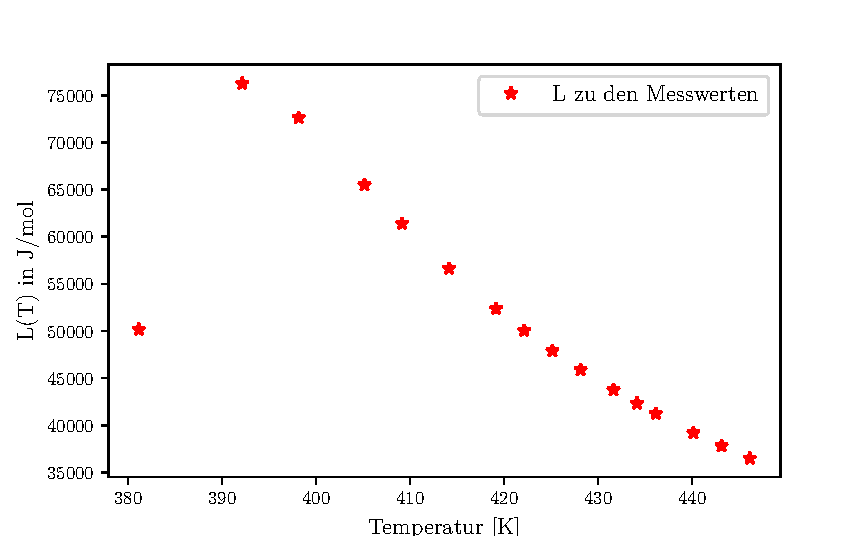
\includegraphics{plot2.pdf}
    \caption{Kurven des Doppelspaltes und des Einfachspaltes}
    \label{fig:verleich}
  \end{figure}